%%%%% Document Setup %%%%%%%%

\documentclass[12pt, onecolumn]{revtex4}    % Font size (12pt) and column number (one or two).

\usepackage[a4paper, left=2.5cm, right=2.5cm, top=2.5cm, bottom=2.5cm]{geometry}  % Defines paper size and margin length

\renewcommand{\baselinestretch}{1}     % Defines the line spacing

\usepackage{subcaption}

\usepackage[font=small, labelfont=bf]{caption}                      % Defines caption font size and caption title bolded
\captionsetup[figure]{justification=justified, singlelinecheck, font=small} 
\captionsetup[table]{justification=justified, singlelinecheck=off, font=small} 
\captionsetup{compatibility=false}

\usepackage{graphics,graphicx,epsfig,ulem}	% Makes sure all graphics works
\usepackage{amsmath} 						% Adds mathematical features for equations

\usepackage{fancyhdr}

\usepackage{textcomp}

\usepackage{tabularx}

\def\thesection{\arabic{section}}
\def\thesubsection{\alph{subsection}}

\def\bibsection{\section*{References}}        % Position reference section correctly

%%%%% Document %%%%%
\begin{document}                     

\title{Testing the Milankovitch-Croll hypothesis using $\delta^{18}$O foram data} 
\maketitle
%\thispagestyle{plain} % produces page number for front page

\vspace{-4ex}

The Milankovitch-Croll hypothesis suggests that changes in Earth's orbit around the Sun leads to fluctuations in solar insolation therefore affecting Earth's planetary climate \cite{ruddiman_climate}. The hypothesis can be explored by analysing proxy data (deep ocean sediment cores) and Earth orbital data. Sediment cores provide a $\delta^{18}$O ratio trace in benthic foram shells to measure the global temperature fluctuations and global ice volume across history \cite{droxler_climate}. \\

% cite the original Milankovitch paper for the reference on what the hypothesis is?

Defined from laboratory experiments, a $\sim 5^{\circ}\mathrm{C}$ temperature increase leads to an $\sim 1$\textperthousand\ decrease in the $\delta^{18}$O. In the case of ice-sheets melting, more $^{16}$O would be released into the oceans, therefore reducing the ratio. Sediment core data for an early (0.0 to 1.0 Myr BP) and late (4.0 to 5.0 Myr BP) period of Earth's history (Fig.~\ref{fig:foram_data}) indicates that in the more recent age the temperature had been varying more dramatically in line with the amplitude of the $\delta^{18}$O. This would have lead to longer periods of cooling and with a cooler climate, there would have been a larger amount of global ice. In both sets of $\delta^{18}$O data, there features a sinusoidal-like trend. Whilst the older data has a smaller amplitude, it can still be suggested that the glacial-interglacial events are a normal part of Earth's planetary climate cycle and that there could be an origin from the cyclical Earth-Sun orbit relationship. \\

In analysing the astrophysical data there are three concepts to consider \cite{ruddiman_climate}: (i) eccentricity, (ii) precession, and (iii) obliquity. The former describes the ellipticity of the Earth's orbit around the Sun, it's effect on insolation however is not entirely independent as the eccentricity depends on the orbital angle between the solstices and the position of perihelion/aphelion. A precessional index value can be produced with $\chi= \varepsilon \sin{\omega}$, where $\varepsilon$ is the eccentricity and $\omega$ is the angle. Finally the obliquity can be defined as the value which describes the degree of tilt of the Earth's axis relative to the orbital plane.  \\

To evaluate and verify that our orbital data agrees with literature, two statistical techniques can be applied in PAST3 \cite{past3}: (i) \textit{wavelet transform} (WT) analysis, and (ii) \textit{REDFIT} analysis. Processing the orbital data with these two tools produces results (Table \ref{table:final_results}) which have an average $\sim 96 \%$ agreement when compared with literature wavelengths. Knowing that the methods are valid and that they produce accurate results, the $\delta^{18}$O foram data can be subsequently analysed.  \\

Initially looking at the data, there is a signal which could be attributed to the obliquity as there are wavelengths of 41.1 ka (REDFIT) and 38.9 ka (WT) which are comparable to the actual value of 41 ka. However from WT analysis (Fig.~\ref{fig:wa_d18o}) this obliquity is only prevalent from 0.15 Myr to 1.28 Myr BP. Beyond this there is a complete disconnect which could be attributed to the rise of eccentricity as the wavelengths are $\sim 100$ ka. Using WT, from $\sim 1.28$ Myr to 4.80 Myr BP there contains a signal of 96.0 ka, and similarly with REDFIT a wavelength of 96.3 ka can be found.  It is therefore not unreasonable to search for a third signal which then can be associated with the perihelion longitude. Consequently one signal is apparent, 23.7 ka, but it can only be seen with REDFIT analysis. The lack of this in WT could be attributed to the fact that the data is dominated and spanned by an ``extended eccentricity signal''. Before 1.28 Myr BP and after 4.80 Myr BP, there are additional wavelengths of 945.5 ka and 1247.6 ka. It could be suggested that the latter signal is related to the eccentricity as it is a multiple of the strongest yet missing component of eccentricity forcing \cite{berger_climate}, 413 ka. More analysis and research would be required to verify or disprove this. \\

Through various analyses of the $\delta^{18}$O data, it can therefore be implied that that the Milankovitch-Croll hypothesis does contain some merit. However there are various issues and questions which prevent the theory from being fully accepted. \\

One prevailing issue is why do the orbital features in the benthic foram data not span the entirety of the data set? If the hypothesis was to be taken at face value then it would be expected that the signals should be seen across the length of the WT heatmaps (as in Fig.~\ref{fig:wa_orbital_data}). In particular the obliquity only covers $\sim 1.13$ Myr, yet from REDFIT (Fig.~\ref{fig:d18o_redfit}) it was found to be the strongest signal. M.~E.~Raymo et al.~provides a model on how local insolation changes would affect the Antarctic ice sheets from $\sim 1.0$ Myr to 3.0 Myr BP \cite{raymo_plio}. They established that the dominant 41.1 ka obliquity signal could be the result of out-of-phase ice sheet growth at each pole because ice volume changes in each hemisphere would cancel the other out. They further proposed that the long-term cooling from the transition of a land-based to marine-based East Antarctic Ice Sheet would lead to the strengthening of the 23 ka cycles at $\sim 2.0$ Myr. Analysis of our own data does verify this, as whilst there are no smooth horizontal features, there are patches which potentially indicate continued signals. This patchiness could potentially explain the greater variation in ice sheet volume from 0.0 Myr to $\sim 3.0$ Myr BP, as during this earlier period it appears that all three orbital features were ``stacking together'' to affect insolation. \\ 

However, there are other failures of the Milankovitch-Croll model, namely evidence of the \textit{p}CO$_{2}$ levels rising in the last two glacial terminations before the $^{18}$O of the atmosphere \cite{sowers_climate, broecker_terminationii}. This could suggest that \textit{p}CO$_{2}$ is the main driver of glacial-interglacial cycles and not changes in the Earth-Sun orbit. It is more likely though that the CO$_{2}$ could be contributing towards a positive feedback loop which amplifies the Milankovitch-Croll cycles \cite{sigman_atmosphere}. If there are higher levels of CO$_{2}$ in the atmosphere then that means more heat will be trapped due to the Greenhouse Effect, therefore could contribute towards the melting of the ice-sheets. Alternatively, the \textit{p}CO$_{2}$ could be driven by changes in meteorological forcing through the delivery of metal dust to ocean surface, which then results in an acausal correlation between Northern Hemisphere summer insolation and ice volume \cite{archer_pco2}. \\

A final and important issue when considering the viability of the Milankovitch-Croll hypothesis 

\newpage

%\twocolumngrid

\bibliographystyle{unsrt}
\bibliography{practical_2}

\newpage

\section*{Appendices}
\begin{figure}[!h]
\begin{center}
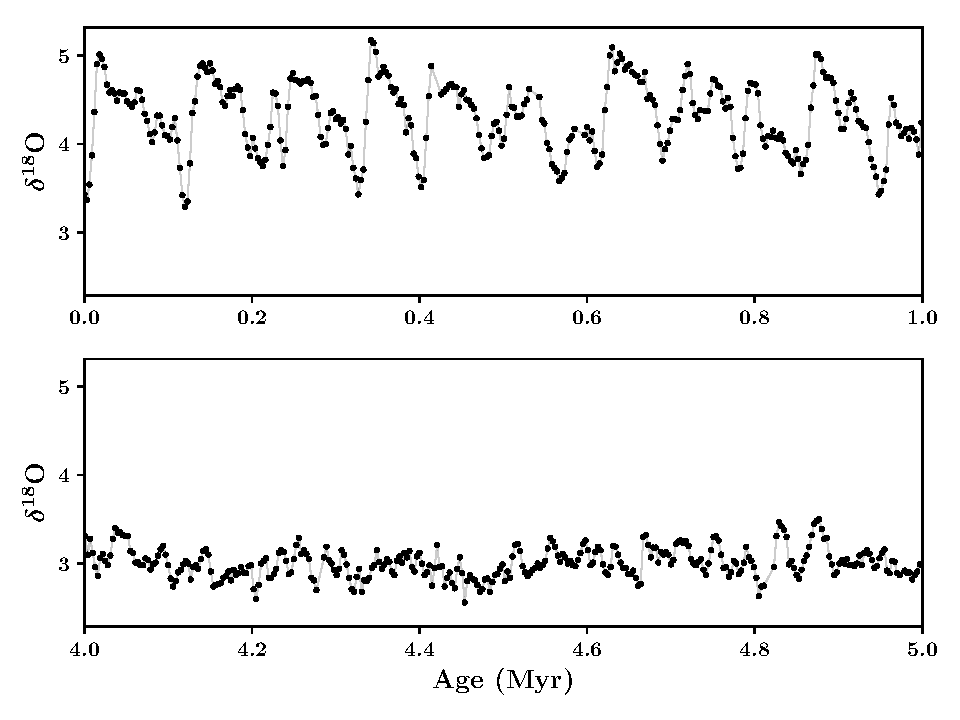
\includegraphics[width=11cm]{figures/foram_data}
\caption[]{Plots of the marine benthic foram $\delta^{18}$O data against age, with increasing time to the right. Both data sets have been taken out of a larger set which spans from 0 Myr to 6 Myr. As we move closer towards the present day, the periodicity and amplitude is larger which implies more extreme temperature variations so longer glacial-interglacials and a larger change in the global ice volume.}
\vspace{-3ex}
\label{fig:foram_data}
\end{center}
\end{figure}

\begin{figure}[!h]
\begin{center}
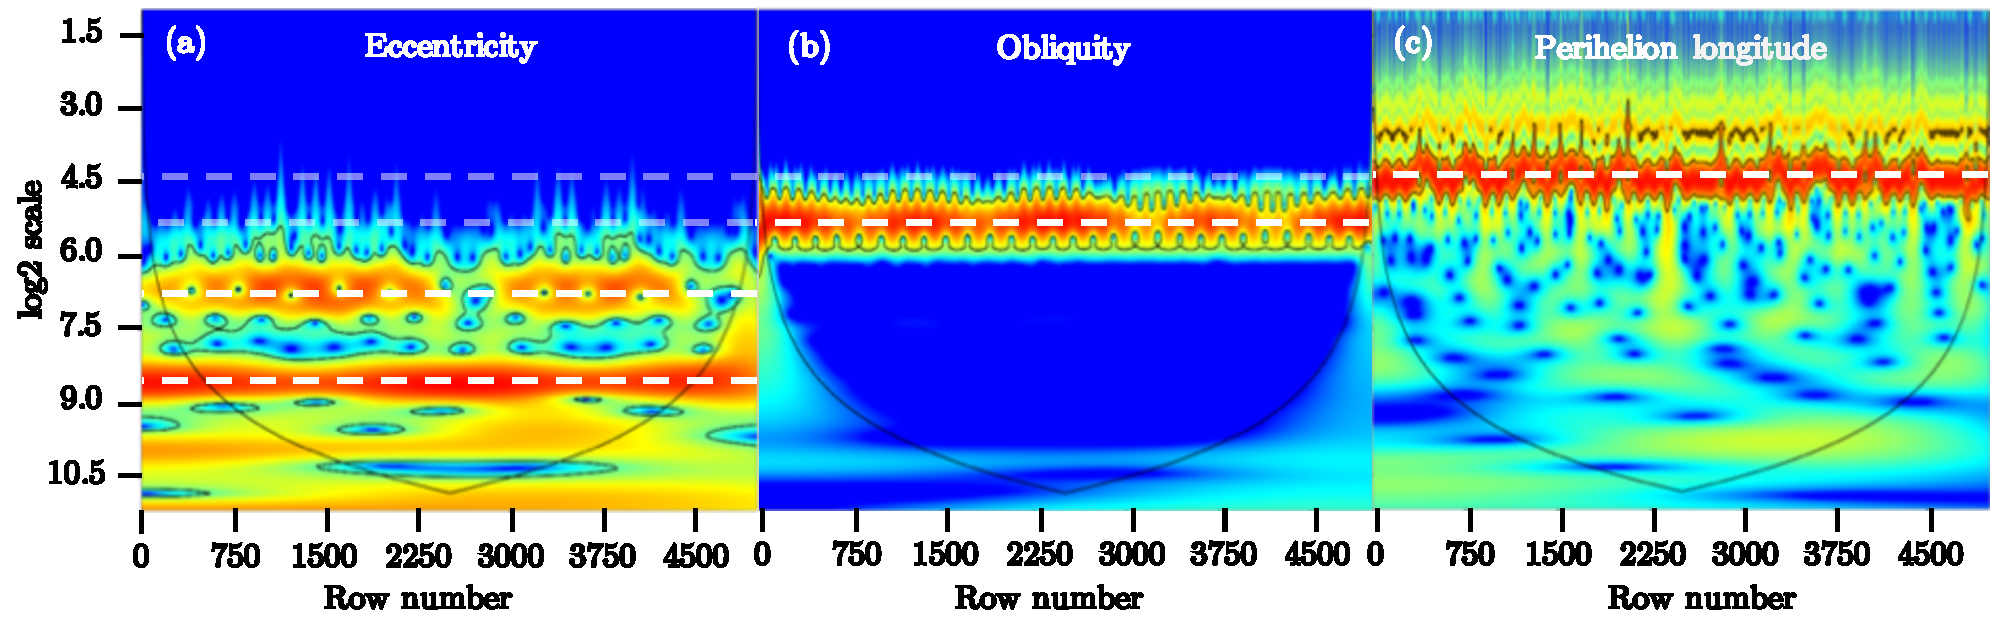
\includegraphics[width=16.2cm]{figures/wa_orbital_data}
\caption[]{The eccentricity, obliquity and perihelion longitude (precession) orbital data which has been processed with the wavelet transform analysis tool in PAST3. The periodicities from the data can be obtained by considering the ``hottest'' areas of each of the heat maps (i.e. the red/orange areas). Values for the wavelength can be found with $2^y \times P$, where $y$ is the y-axis height of the hot region, and $P$ is the period of time between the data points. In Table \ref{table:final_results} we summarise the wavelengths which correspond to the dashed-line heights.}
\vspace{-3ex}
\label{fig:wa_orbital_data}
\end{center}
\end{figure}

\begin{figure}[!h]
\begin{center}
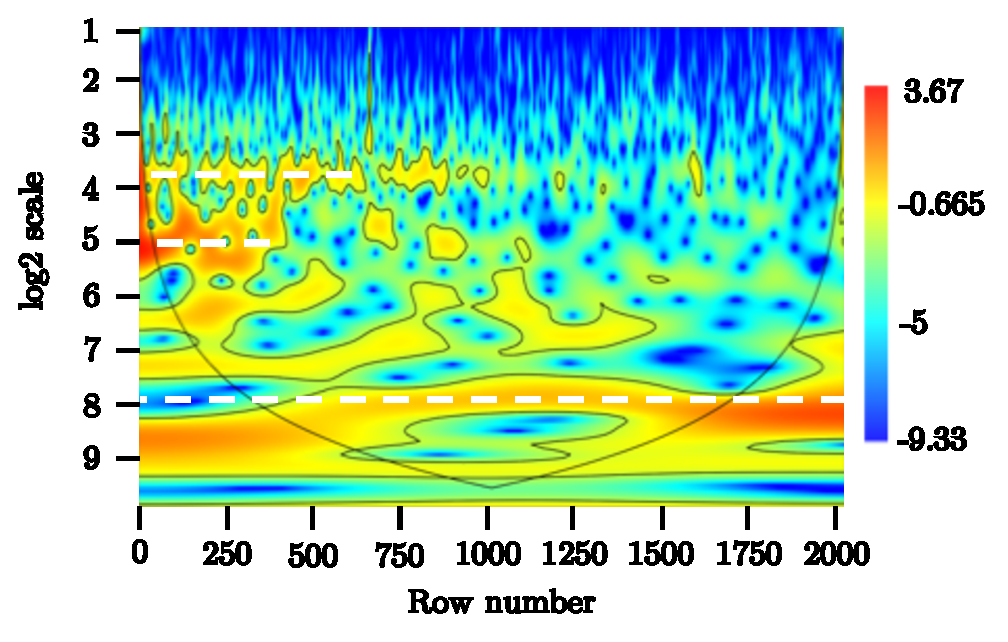
\includegraphics[width=11cm]{figures/wa_d18O.pdf}
\caption[]{The result from applying the PAST3 wavelet transform analysis tool to the $\delta^{18}$O benthic foram data, the wavelengths found are summarised in Table \ref{table:final_results}. The results are similar to those found in the orbital data, which could imply that orbital forcing does have an influence on glacial-interglacial climate.}
\vspace{-3ex}
\label{fig:wa_d18o}
\end{center}
\end{figure}

\begin{figure}[!h]
\begin{center}
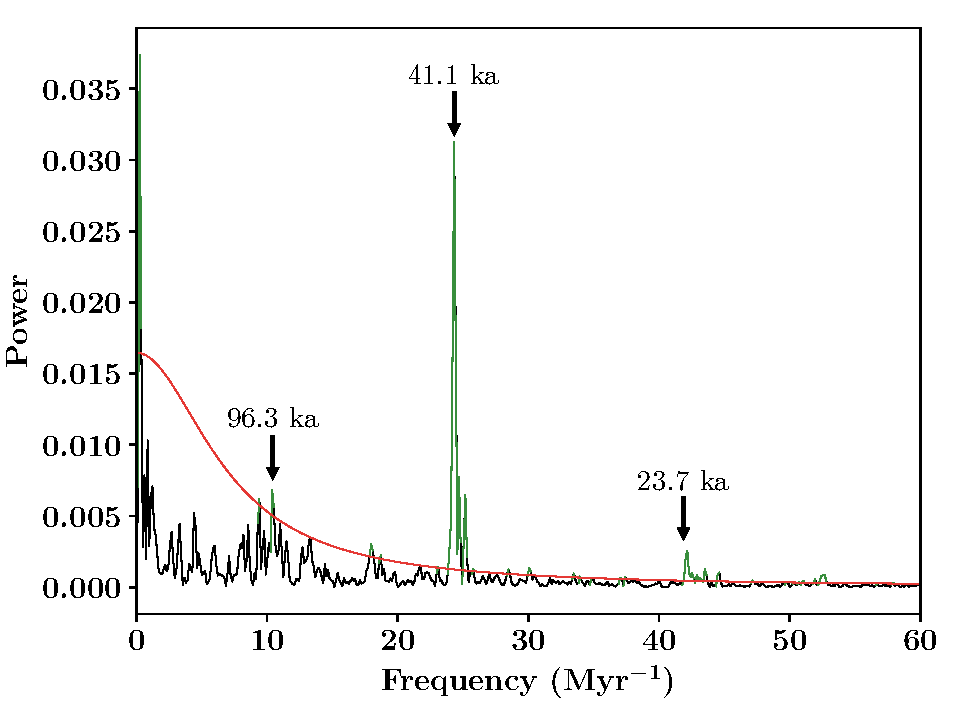
\includegraphics[width=11cm]{figures/d18O_redfit}
\caption[]{The benthic foram $\delta^{18}$O data analysed using the REDFIT spectral analysis tool in PAST3. Three dominant signals can be seen as coloured in green, they are defined as the main signals as they have a height greater than the $95\%$ confidence interval (the red curve). The same results can be found in Table \ref{table:final_results}, and comparing to the ``true'' wavelengths we also find similarities which further strengthens the possibility that the Milankovitch-Croll hypothesis has some validity.}
\vspace{-3ex}
\label{fig:d18o_redfit}
\end{center}
\end{figure}

\begin{table}[h!]
\centering
\begin{tabular}{c@{\hskip 20pt}c@{\hskip 20pt}c@{\hskip 20pt}c} 
 \hline
  & \textbf{Literature (ka)} &\textbf{REDFIT (ka)} & \textbf{WT (ka)} \\ [0.5ex] 
 Eccentricity & 100, 413 & 95.2, 128.2, 416.7 & 89.1, 100.4,  401.7\\
 Perihelion Longitude & 23, 100 & 23.8, 22.2 & 21.1 \\
 Obliquity & 41 & 41.7 & 39.4 \\
 $\delta^{18}$O & & 23.7, 41.1, 96.3  & 38.9, 96.0, 271.5, \\
 & & & 945.5, 1247.6 \\
 \hline
\end{tabular}
\caption{Table showing different sets of wavelength data: the approximate correct wavelengths for the periodicity of the orbital features \cite{campisano_milankovitch}, the results of the REDFIT spectral analysis and Wavelet Transform (WT) analysis on the orbital and benthic foram data. We find that as tools both REDFIT and WT are able to obtain similar periodicities which then agree with the literature values. }
\vspace{-0.5em}
\label{table:final_results}
\end{table}

\end{document}